\chapter{Implementação}
\label{cap:implementacao}

Este capítulo descreve em detalhe a implementação do sistema desenvolvido para análise automatizada de \glspl{ODS} a partir de avaliações associadas a locais físicos. O sistema foi construído em Python 3 e evoluiu de um protótipo específico para uma arquitetura generalizável, capaz de ser parametrizada para diferentes ODS, municípios e modelos de linguagem de grande porte. A implementação passou por três versões principais: a primeira voltada à análise ESG, a segunda composta por modelos específicos para o ODS 9 e o ODS 16, e a terceira consolidada como um motor genérico orientado por arquivos JSON de configuração.

\section{Arquitetura Geral do Sistema}
\label{sec:arq-geral}

O sistema é composto por quatro módulos principais:

\begin{enumerate}
    \item \textbf{Módulo de Configuração}: lê arquivos JSON que especificam o ODS alvo, município, termos de busca, aspectos a analisar, modelos de IA e parâmetros de execução;
    \item \textbf{Módulo de Coleta}: realiza buscas na Google Places API utilizando termos e coordenadas estratégicas do município, coletando avaliações (\textit{reviews}) dos estabelecimentos encontrados;
    \item \textbf{Módulo de Filtragem e Pré-processamento}: aplica filtros hierárquicos de validação geográfica, relevância por tipo de local e qualidade de conteúdo;
    \item \textbf{Módulo de Análise com IA}: envia cada comentário filtrado a uma LLM para classificação de sentimento por aspecto do ODS, geração de justificativas e extração de palavras-chave.
\end{enumerate}

\clearpage

A Figura~\ref{fig:fluxo-pipeline} sintetiza o fluxo operacional da solução, desde a configuração inicial do experimento até a disponibilização dos resultados em \textit{dashboards}.

\begin{figure}[!t]
    \centering
    \caption{Fluxograma da pipeline de análise automatizada de ODS}
    \label{fig:fluxo-pipeline}
    \normalsize
    \setlength{\fboxsep}{6pt}
    \renewcommand{\arraystretch}{1.0}
    \begin{tabular}{c}
        \fbox{\parbox{0.78\textwidth}{\centering \textbf{1. Configuração JSON}\\Definição do ODS, município, dimensões, termos de busca, bases de dados e modelos de IA}}\\[0.18cm]
        $\downarrow$\\[0.18cm]
        \fbox{\parbox{0.78\textwidth}{\centering \textbf{2. Busca no Google Places API}\\Consulta de locais físicos associados aos termos configurados e às coordenadas do município}}\\[0.18cm]
        $\downarrow$\\[0.18cm]
        \fbox{\parbox{0.78\textwidth}{\centering \textbf{3. Detalhes do Local}\\Coleta de nome, endereço, coordenadas, avaliação média e comentários públicos disponíveis}}\\[0.18cm]
        $\downarrow$\\[0.18cm]
        \fbox{\parbox{0.78\textwidth}{\centering \textbf{4. Filtros}\\Validação geográfica, deduplicação, comprimento mínimo, relevância semântica e adequação ao ODS}}\\[0.18cm]
        $\downarrow$\\[0.18cm]
        \fbox{\parbox{0.78\textwidth}{\centering \textbf{5. Análise com LLM}\\Classificação de sentimento por aspecto, justificativa, confiança, palavras-chave e indicação de problema}}\\[0.18cm]
        $\downarrow$\\[0.18cm]
        \fbox{\parbox{0.78\textwidth}{\centering \textbf{6. Saída JSON}\\Geração de registros estruturados com metadados, análises individuais e estatísticas agregadas}}\\[0.18cm]
        $\downarrow$\\[0.18cm]
        \fbox{\parbox{0.78\textwidth}{\centering \textbf{7. Diagnóstico}\\Síntese textual automática por ODS e por dimensão, com pontos críticos e recomendações}}\\[0.18cm]
        $\downarrow$\\[0.18cm]
        \fbox{\parbox{0.78\textwidth}{\centering \textbf{8. Dashboard}\\Visualização interativa dos indicadores, mapas, sentimentos, dimensões problemáticas e diagnósticos}}
    \end{tabular}
    \legend{Fonte: Elaborado pelo autor (2025).}
\end{figure}

\section{Evolução da Implementação}
\label{sec:evolucao}

\subsection{Primeira Versão: Modelo de Análise ESG}
\label{subsec:v1}

A primeira versão do sistema consistiu em um modelo de análise ESG, estruturado para avaliar comentários públicos segundo três dimensões: Ambiental, Social e Governança. Essa etapa teve caráter exploratório e permitiu validar a integração entre a Google Places API, responsável pela coleta de avaliações associadas a estabelecimentos e locais físicos, e os modelos de linguagem utilizados para classificar sentimentos, extrair palavras-chave e gerar justificativas textuais.

Nessa versão, cada dimensão possuía um conjunto próprio de aspectos. A dimensão ambiental considerava temas como infraestrutura urbana, saneamento, qualidade ambiental, conservação, mobilidade sustentável e conforto urbano. A dimensão social analisava inclusão, acessibilidade, segurança, saúde, cultura, trabalho e coesão comunitária. A dimensão de governança contemplava transparência, organização, gestão de recursos, participação, conformidade, ética e prestação de contas.

Apesar de funcional, essa primeira versão ainda possuía limitações importantes. Os termos de busca, os aspectos de análise e a estrutura de saída estavam fortemente vinculados ao domínio ESG, exigindo adaptação manual para aplicação direta em um ODS específico. Ainda assim, ela demonstrou que avaliações públicas não estruturadas poderiam ser convertidas em dados analíticos estruturados por meio de \glspl{LLM}.

\subsection{Segunda Versão: Modelos Específicos para ODS 9 e ODS 16}
\label{subsec:v2}

A segunda versão deslocou o foco da análise ESG para objetivos específicos da Agenda 2030, com implementações dedicadas ao ODS 9 (Indústria, Inovação e Infraestrutura) e ao ODS 16 (Paz, Justiça e Instituições Eficazes). Nessa etapa, cada ODS passou a ter seus próprios termos de busca, dimensões analíticas, filtros semânticos e prompts especializados.

Para o ODS 9, o modelo foi estruturado em sete dimensões: Infraestrutura Resiliente e Moderna; Transporte Público e Mobilidade; Acesso à Tecnologia e Informação; Inovação e Pesquisa; Industrialização Inclusiva e Sustentável; Eficiência Energética; e Valorização da Micro e Pequena Empresa. Para o ODS 16, foram definidas dimensões relacionadas a Instituições Eficazes, Direitos Humanos, Segurança Pública, Acesso à Justiça, Transparência, Participação Cidadã e Proteção de Grupos Vulneráveis.

Essa versão também introduziu campos booleanos para indicar se cada comentário contribuía para o baixo desempenho do município no respectivo ODS. Assim, além da classificação de sentimento, o sistema passou a produzir métricas quantitativas diretamente relacionadas ao problema de pesquisa, como o percentual de análises que indicavam fragilidades em infraestrutura, transporte, serviços institucionais ou segurança pública.

\subsection{Terceira Versão: Motor Genérico via Configuração JSON}
\label{subsec:v3}

A terceira versão consolidou a arquitetura em um motor genérico parametrizado por arquivos JSON de configuração. Em vez de manter um script distinto para cada ODS, o sistema passou a receber como entrada um arquivo que define o ODS analisado, o município, as dimensões avaliadas, os termos de busca, as chaves das bases de dados e os modelos de IA disponíveis. Esta arquitetura tornou o sistema extensível sem alterações diretas no código-fonte.

Cada arquivo de configuração especifica:

\begin{itemize}
    \item \textbf{Identificação do ODS}: número, nome e descrição;
    \item \textbf{Município alvo}: nome, estado, coordenadas estratégicas de busca e raio em metros;
    \item \textbf{Termos de busca}: lista de palavras-chave para cada categoria relevante ao ODS;
    \item \textbf{Aspectos a analisar}: os 7 aspectos do ODS com seus tópicos associados;
    \item \textbf{Modelos de IA}: lista de modelos LLM configurados (Gemini ou Perplexity), com chaves de API resolvidas via arquivo \texttt{env.properties};
    \item \textbf{Parâmetros de execução}: metas de análises, limites de rate, pausas entre requisições.
\end{itemize}

O Código~\ref{lst:config-ods9} apresenta um trecho representativo do arquivo de configuração para o ODS 9:

\begin{lstlisting}[language=,caption={Trecho do arquivo de configuração ODS 9 (ods9\_config.json)},label={lst:config-ods9}]
{
  "ods": {
    "numero": 9,
    "nome": "Indústria, Inovação e Infraestrutura",
    "sigla": "ODS 9"
  },
  "municipio": {
    "nome": "Mossoró",
    "estado": "RN",
    "coordenadas_estrategicas": [
      {"lat": -5.1875, "lng": -37.3444, "descricao": "Centro"},
      {"lat": -5.1650, "lng": -37.3600, "descricao": "Zona Norte"},
      {"lat": -5.2100, "lng": -37.3200, "descricao": "Zona Sul"}
    ],
    "raio_busca_metros": 15000
  },
  "termos_busca": {
    "infraestrutura_transporte": [
      "rodoviária Mossoró", "aeroporto Mossoró", "terminal rodoviário"
    ],
    "infraestrutura_urbana": [
      "rua pavimentação Mossoró", "ponte viaduto Mossoró"
    ],
    "tecnologia_telecomunicacoes": [
      "provedor internet Mossoró", "operadora telefonia Mossoró"
    ]
  }
}
\end{lstlisting}

A versão genérica também adicionou suporte nativo a múltiplos provedores de \gls{LLM}: Google Gemini (modelos Flash e Pro) e Perplexity (modelos Sonar e Sonar Pro). A seleção do modelo é realizada interativamente no início da execução ou pode ser pré-configurada no arquivo JSON. O mecanismo de \textit{fallback} automático garante que, caso o modelo principal retorne erro, o sistema tente automaticamente o próximo modelo disponível na configuração.

A resolução de credenciais de API é feita por um mecanismo centralizado que lê variáveis de ambiente ou o arquivo \texttt{env.properties} na raiz do projeto, sem expor chaves sensíveis no código-fonte. O sistema também implementa um formulário HTML para geração interativa de novos arquivos de configuração, facilitando a extensão para novos municípios e ODS.

\section{Módulo de Coleta de Dados}
\label{sec:coleta}

\subsection{Google Places API como Fonte de Dados}
\label{subsec:google-places}

O módulo de coleta utiliza a Google Places API como fonte primária de dados. Para cada termo de busca definido na configuração, o sistema realiza buscas em múltiplas coordenadas estratégicas do município, com raio configurável (padrão: 15 km). Para cada lugar encontrado, o sistema obtém os detalhes completos, incluindo nome, endereço, coordenadas geográficas, avaliação média e todas as avaliações textuais disponíveis.

O Código~\ref{lst:busca-lugares} apresenta a função responsável pela busca de estabelecimentos:

\begin{lstlisting}[language=Python,caption={Função de busca de lugares na Google Places API},label={lst:busca-lugares}]
def buscar_lugares_mossoro(termo: str, coordenadas: Dict[str, float]) -> List[Dict]:
    url = "https://maps.googleapis.com/maps/api/place/textsearch/json"
    params = {
        'query': f"{termo} Mossoró RN",
        'location': f"{coordenadas['lat']},{coordenadas['lng']}",
        'radius': RADIUS,
        'key': GOOGLE_PLACES_API_KEY,
        'language': 'pt-BR'
    }
    try:
        response = requests.get(url, params=params)
        data = response.json()
        if data.get('status') == 'OK':
            return data.get('results', [])
        return []
    except Exception as e:
        print(f"Erro na busca por '{termo}': {e}")
        return []
\end{lstlisting}

\subsection{Análise de Fontes Alternativas de Dados}
\label{subsec:fontes-alternativas}

Além da Google Places API, foram avaliadas outras fontes potenciais de dados não estruturados, especialmente redes sociais. No entanto, essas alternativas apresentaram limitações técnicas, financeiras e operacionais que inviabilizaram sua adoção no escopo desta pesquisa.

No caso do Instagram, a API oficial impõe restrições relevantes para coleta automatizada de comentários, especialmente quando se busca conteúdo público associado a locais ou estabelecimentos. Além disso, o acesso a determinados recursos exige configuração formal de aplicativo, política de privacidade, ícone, submissão para análise e aprovação individual de permissões pela Meta. Essas exigências aumentam a complexidade operacional e não garantem acesso efetivo aos comentários necessários para a análise.

O Facebook também foi avaliado, mas o acesso ficou limitado a informações de páginas administradas pelo próprio pesquisador ou a dados com permissões restritas. A coleta de informações de páginas de terceiros e comentários públicos depende de permissões específicas e aprovação da Meta, o que reduz a viabilidade de uso em uma pesquisa que exige dados comparáveis entre diferentes locais públicos.

A plataforma X/Twitter foi considerada como alternativa; contudo, seu uso apresenta barreiras financeiras significativas, uma vez que o acesso à API com volume e funcionalidades adequadas para mineração de dados tornou-se pago. Já o Threads foi descartado por ainda apresentar uma API em estágio de amadurecimento, com limitações para coleta estruturada e ampla de comentários públicos.

Diante dessas restrições, optou-se pela Google Places API como fonte principal de dados, por disponibilizar avaliações diretamente associadas a locais físicos, incluindo estabelecimentos públicos, equipamentos urbanos, instituições e serviços municipais. Essa característica é especialmente relevante para esta pesquisa, pois permite relacionar percepções dos cidadãos a dimensões concretas dos \glspl{ODS} no território municipal.

\subsection{Gerenciamento de Rate Limiting}
\label{subsec:rate-limit}

Para respeitar os limites de requisição das APIs utilizadas, o sistema implementa pausas estratégicas configuráveis: 1 segundo entre análises de \textit{reviews} individuais, 2 segundos entre lugares processados e 3 segundos entre buscas de termos distintos. O controle de deduplicação evita reprocessar o mesmo estabelecimento em buscas de termos diferentes.

\section{Módulo de Filtragem e Pré-processamento}
\label{sec:filtragem}

\subsection{Filtragem Hierárquica}
\label{subsec:filtros}

O módulo de filtragem aplica cinco camadas de validação para garantir que apenas comentários relevantes e de qualidade sejam enviados para análise. A ordem dos filtros é importante: filtros mais baratos computacionalmente são aplicados primeiro.

\textbf{Filtro 1 -- Validação Geográfica}: verifica se o estabelecimento está localizado no município alvo, verificando a presença do nome do município no endereço ou nome do estabelecimento retornado pela API. Esta validação é necessária pois buscas com raio amplo podem capturar estabelecimentos de municípios vizinhos.

\textbf{Filtro 2 -- Comprimento Mínimo}: descarta comentários com menos de 20 caracteres, que geralmente não contêm informação analiticamente útil.

\textbf{Filtro 3 -- Relevância Geográfica do Conteúdo}: elimina comentários que mencionam explicitamente outras cidades sem referenciar o município alvo, evitando que avaliações sobre filiais em outras localidades contaminem a análise.

\textbf{Filtro 4 -- Relevância Semântica por ODS}: verifica se o comentário contém pelo menos um termo relacionado aos aspectos do ODS analisado. Esta verificação é dispensada para locais de infraestrutura crítica (rodoviárias, aeroportos, delegacias), onde qualquer experiência do usuário é considerada relevante.

\textbf{Filtro 5 -- Filtros Específicos por ODS}: para o ODS 16, comentários de caráter histórico, turístico ou puramente comercial são descartados, pois não refletem a situação atual dos serviços públicos.

\subsection{Confiabilidade dos Reviews e Mitigação de Vieses}
\label{subsec:confiabilidade-reviews}

Embora as avaliações disponibilizadas pela Google Places API constituam uma fonte rica de dados perceptivos, elas não devem ser tratadas como representação estatisticamente perfeita da opinião da população. Esse tipo de dado pode apresentar viés de seleção, uma vez que apenas uma parcela dos usuários registra avaliações públicas e essa parcela tende a ser composta por pessoas com maior motivação para relatar experiências marcantes, sejam elas positivas ou negativas. Em particular, usuários insatisfeitos podem ter maior propensão a comentar, o que pode aumentar a presença de avaliações críticas em determinados estabelecimentos.

Outra limitação relevante refere-se à possibilidade de avaliações falsas, duplicadas, desatualizadas ou motivadas por interesses particulares. Embora a plataforma Google adote mecanismos próprios de moderação, o sistema desenvolvido nesta pesquisa não possui acesso aos critérios internos de detecção de autenticidade nem consegue garantir, de forma independente, que todos os comentários coletados correspondem a experiências reais. Portanto, a autenticidade total dos \textit{reviews} não pode ser assegurada apenas pelo pipeline implementado.

Para reduzir esses riscos, o sistema aplica camadas sucessivas de filtragem e pré-processamento antes da análise por \gls{LLM}. A validação geográfica verifica se o estabelecimento pertence ao município investigado; a deduplicação evita reprocessar o mesmo local em buscas diferentes; o filtro de comprimento mínimo remove comentários sem conteúdo analítico suficiente; a verificação de relevância semântica seleciona apenas textos relacionados ao ODS analisado; e os filtros específicos por objetivo descartam avaliações cujo conteúdo não representa a situação atual do serviço ou equipamento público. Essas etapas reduzem ruídos e inconsistências, mas não eliminam completamente vieses de origem dos dados.

Dessa forma, os resultados obtidos devem ser interpretados como um sinal perceptivo complementar aos indicadores oficiais, e não como substitutos desses indicadores. A contribuição da abordagem está em capturar percepções situadas, associadas a locais físicos específicos, que podem revelar gargalos, recorrências e pontos críticos não evidenciados por métricas agregadas. A interpretação dos diagnósticos deve, portanto, ocorrer por triangulação com fontes oficiais, conhecimento especializado e, quando possível, validação manual ou avaliação por especialistas.

\section{Módulo de Análise com Inteligência Artificial}
\label{sec:analise-ia}

\subsection{Prompt Engineering para Análise por Aspecto}
\label{subsec:prompt}

Para cada comentário aprovado pelos filtros, o sistema constrói um prompt estruturado que instrui o LLM a realizar análise por aspecto (\textit{aspect-based sentiment analysis}). O prompt inclui o texto do comentário, o nome do estabelecimento, o ODS analisado, o contexto de que Mossoró possui pontuação muito baixa naquele ODS, e a lista completa dos aspectos a analisar com seus tópicos associados.

O formato de saída solicitado é JSON estruturado, contendo para cada aspecto: classificação de sentimento (Positivo, Negativo, Neutro ou Não mencionado), \textit{score} de confiança (0,0 a 1,0), justificativa curta em até 15 palavras, até três palavras-chave e um indicador booleano de problema. O Código~\ref{lst:analise-ods9} mostra a estrutura principal da função de análise para o ODS 9:

\begin{lstlisting}[language=Python,caption={Estrutura da função de análise de aspectos ODS 9},label={lst:analise-ods9}]
def analisar_aspectos_ods9(texto: str, nome_lugar: str, modelo: Dict = None) -> Dict:
    prompt = f"""
    Aja como analista especializado em ODS 9 (Indústria, Inovação e Infraestrutura).
    
    COMENTÁRIO: "{texto}"
    LOCAL: "{nome_lugar}"
    CIDADE: Mossoró-RN (pontuação MUITO BAIXA no ODS 9)
    
    Analise os seguintes aspectos e retorne JSON estruturado:
    1. Infraestrutura Resiliente e Moderna
    2. Transporte Público e Mobilidade
    3. Acesso à Tecnologia e Informação
    4. Inovação e Pesquisa
    5. Industrialização Inclusiva e Sustentável
    6. Eficiência Energética e Energia Sustentável
    7. Valorização da Micro e Pequena Empresa
    ...
    """
    try:
        if modelo['tipo'] == 'gemini':
            gemini_model = genai.GenerativeModel(modelo['model_id'])
            response = gemini_model.generate_content(prompt)
            response_text = response.text
        response_text = re.sub(r'```json\s*', '', response_text)
        response_text = re.sub(r'```\s*', '', response_text)
        json_match = re.search(r'(\{.*\})', response_text, re.DOTALL)
        if json_match:
            return json.loads(json_match.group(1))
    except Exception as e:
        return {"erro": str(e)}
\end{lstlisting}

\subsection{Geração de Diagnósticos Agregados}
\label{subsec:diagnosticos}

Após a análise individual de todos os comentários, o sistema executa uma segunda etapa de síntese: para cada ODS analisado, um novo prompt é enviado ao LLM contendo as estatísticas agregadas (distribuição de sentimentos, contagem de problemas por dimensão, aspectos mais frequentes e palavras-chave predominantes). O modelo retorna um diagnóstico estruturado em seis seções: identificação das causas do baixo desempenho, análise por dimensão, pontos críticos prioritários, impacto social e econômico, recomendações estratégicas e conclusão.

Para cada ODS, diagnósticos adicionais são gerados para cada dimensão individualmente, detalhando a situação atual, o impacto no ODS geral e recomendações específicas para aquela dimensão.

\section{Estrutura de Saída e Integração com Dashboard}
\label{sec:saida}

Os resultados são salvos em arquivos JSON com nome padronizado contendo três seções principais:

\begin{itemize}
    \item \textbf{meta\_informacoes}: total de análises, problemas detectados, percentuais, data da coleta e contexto do ODS;
    \item \textbf{conclusao\_geral\_diagnostico}: texto do diagnóstico geral gerado pela IA;
    \item \textbf{analises\_ods}: \textit{array} com todos os registros individuais, incluindo dados do estabelecimento, análise por aspecto e texto original do \textit{review}.
\end{itemize}

Os arquivos JSON resultantes foram utilizados como fonte de dados para dashboards interativos, permitindo visualização geográfica dos problemas, filtros por tipo de estabelecimento, análise das dimensões do ODS e consulta aos diagnósticos textuais gerados pela IA.

\section{Generalização para Múltiplos ODS}
\label{sec:generalizacao-multiplos-ods}

Cabe esclarecer, de início, que o estudo de caso validado desta dissertação restringe-se aos ODS 9 e 16 em Mossoró-RN, únicos objetivos para os quais foram realizadas coletas em escala e análises aprofundadas (Capítulo~\ref{cap:resultados}). Os ODS 3 e 4 foram incorporados exclusivamente como exercício de generalização, com o propósito de testar se a arquitetura baseada em configuração descrita na Seção~\ref{subsec:v3} de fato permite estender a análise a outros objetivos da Agenda 2030 sem alteração do código-fonte. Não se trata, portanto, de resultados sobre saúde ou educação, mas de evidência de que o motor genérico opera além do par de objetivos validado.

Para esse teste, foram elaborados arquivos de configuração para o ODS 3 (Saúde e Bem-estar) e para o ODS 4 (Educação de Qualidade), denominados \texttt{ods3\_config.json} e \texttt{ods4\_config.json}, gerados com o auxílio do formulário interativo descrito na Seção~\ref{sec:formulario-config}, que dispensa a edição manual do JSON. Esses arquivos seguem exatamente a mesma estrutura dos arquivos utilizados no estudo de caso principal, alterando apenas os parâmetros específicos de cada objetivo: identificação do ODS, termos de busca, palavras-chave de filtragem, dimensões de análise, chaves de saída do JSON e \textit{prompts} especializados.

Para o ODS 3, foram parametrizadas sete dimensões alinhadas às metas do objetivo: Cobertura Vacinal; Mortalidade e Saúde Mental; Saúde Materno-Infantil; Doenças Transmissíveis; Doenças Crônicas e Mortalidade; Atenção Primária e UBS; e Promoção da Saúde e Bem-estar. Os termos de busca passaram a contemplar equipamentos públicos de saúde, como unidades básicas de saúde, hospitais, maternidades, clínicas e postos de vacinação. Para o ODS 4, as sete dimensões definidas foram: Educação Inclusiva e Igualitária; Educação Básica e Acesso; Capacitação e Empoderamento; Direitos Humanos e Desenvolvimento Sustentável na Educação; Qualidade do Ensino e Infraestrutura Educacional; Oportunidades para Pessoas Vulneráveis; e Formação Técnica e Superior, com termos de busca voltados a escolas, creches, universidades, bibliotecas e cursos técnicos.

As execuções foram realizadas pelo motor genérico (\texttt{ods\_analise\_generica.py}), sem qualquer alteração no código-fonte. A Tabela~\ref{tab:generalizacao-ods} resume os resultados quantitativos obtidos nessas execuções exploratórias.

\begin{table}[h!]
    \centering
    \caption{Execuções exploratórias do motor genérico para ODS 3 e ODS 4}
    \label{tab:generalizacao-ods}
    \begin{tabular}{llccc}
        \hline
        \textbf{ODS} & \textbf{Cidade} & \textbf{Análises} & \textbf{Problemas} & \textbf{\% problemas} \\
        \hline
        ODS 3 & Natal-RN & 25 & 19 & 76,0\% \\
        ODS 3 & Fortaleza-CE & 50 & 45 & 90,0\% \\
        ODS 4 & Natal-RN & 25 & 16 & 64,0\% \\
        \hline
    \end{tabular}
    \legend{Fonte: Elaborado pelo autor (2026).}
\end{table}

É importante delimitar o escopo dessas execuções. A validação metodológica completa da abordagem, com coleta em larga escala, análise das dimensões e verificação manual de amostras, foi realizada apenas para os ODS 9 e 16, no estudo de caso de Mossoró-RN; somente esses dois objetivos dispõem de dados em volume suficiente para sustentar análise e diagnóstico. As execuções com os ODS 3 e 4 tiveram caráter exclusivo de verificação de viabilidade técnica: seu propósito foi demonstrar que o pipeline completo (coleta, filtragem, análise por aspecto, geração de JSON e diagnóstico automatizado) executa corretamente para outros objetivos mediante simples troca do arquivo de configuração, com volumes de coleta deliberadamente reduzidos para controlar custos de API. Os percentuais apresentados na Tabela~\ref{tab:generalizacao-ods}, portanto, não constituem diagnósticos validados desses municípios nem conclusões sobre saúde ou educação, mas tão somente evidências de que a generalização para novos objetivos é operacionalmente possível.

\section{Generalização Geográfica}
\label{sec:generalizacao-geografica}

De forma análoga, e também em caráter estritamente exploratório, a capacidade de replicação da análise em outros municípios foi verificada executando os modelos dos ODS 9 e 16 -- estes sim validados em Mossoró-RN -- em quatro capitais do Nordeste: Natal-RN, Fortaleza-CE, João Pessoa-PB e Salvador-BA. Nessas execuções, alterou-se apenas o parâmetro de localidade (cidade e estado), mantendo inalterados as dimensões de análise, os filtros semânticos e os \textit{prompts} de cada objetivo. Vale esclarecer que a aplicação dos modelos dos ODS 9 e 16 a essas outras cidades não configura análise validada desses municípios.

Cada execução gerou um arquivo de análise no mesmo formato padronizado descrito na Seção~\ref{sec:saida}, seguindo a convenção de nomenclatura utilizada nos outros arquivos gerados. Essa padronização permite que os arquivos de diferentes municípios sejam carregados diretamente no dashboard unificado, descrito na Seção~\ref{sec:dashboards-publicos}, sem qualquer conversão. A Tabela~\ref{tab:generalizacao-geografica} resume as execuções realizadas.

\begin{table}[h!]
    \centering
    \caption{Execuções exploratórias dos modelos ODS 9 e ODS 16 em outras cidades}
    \label{tab:generalizacao-geografica}
    \begin{tabular}{llccc}
        \hline
        \textbf{ODS} & \textbf{Cidade} & \textbf{Análises} & \textbf{Problemas} & \textbf{\% problemas} \\
        \hline
        ODS 9 & Fortaleza-CE & 10 & 9 & 90,0\% \\
        ODS 16 & João Pessoa-PB & 10 & 9 & 90,0\% \\
        ODS 16 & Salvador-BA & 5 & 5 & 100,0\% \\
        \hline
    \end{tabular}
    \legend{Fonte: Elaborado pelo autor (2026).}
\end{table}

Assim como na generalização para múltiplos ODS, essas execuções utilizaram amostras intencionalmente pequenas, suficientes para confirmar que a coleta na Google Places API, a filtragem hierárquica e a análise com IA funcionam em diferentes contextos urbanos, mas insuficientes para sustentar conclusões substantivas sobre esses municípios. Com dito anteriormente, a análise aprofundada e validada ficou restrita a Mossoró-RN.

\section{Formulário Interativo de Configuração}
\label{sec:formulario-config}

Como a extensão do sistema a novos contextos depende exclusivamente da criação de arquivos de configuração JSON, foi desenvolvido um formulário web interativo (\texttt{formulario\_config\_ods.html}) para geração assistida desses arquivos, eliminando a necessidade de edição manual e reduzindo a barreira de entrada para usuários não técnicos, como gestores públicos e pesquisadores de outras áreas.

O formulário é uma página estática em HTML, CSS e JavaScript, organizada em blocos que espelham a estrutura do arquivo de configuração: seleção visual do ODS; localidade (município e estado); configuração geral (pontuação atual no IDSC-BR, limite de análises e rótulo do tipo de local); termos de busca no Google Places; dimensões de análise, com nome e tópicos associados; chaves de saída do JSON; e bases de dados, com os nomes das variáveis de ambiente que armazenam as chaves de API. Campos obrigatórios são validados antes da geração, e as dimensões podem ser adicionadas, editadas ou removidas dinamicamente. A Figura~\ref{fig:formulario-config-ods} apresenta a interface do formulário.

\begin{figure}[H]
    \centering
    \caption{Formulário web para geração de arquivos de configuração ODS}
    \label{fig:formulario-config-ods}
    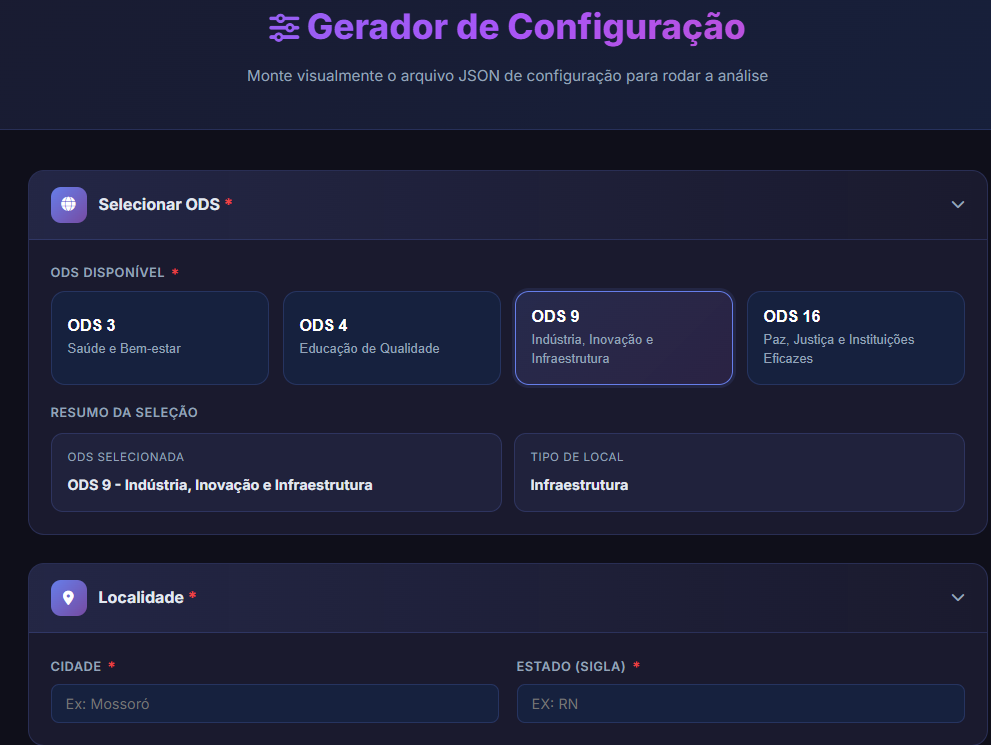
\includegraphics[width=0.70\textwidth]{figuras/formulario-config-ods}
    \legend{Fonte: Elaborado pelo autor (2026).}
\end{figure}

O fluxo de uso completo compreende quatro etapas:

\begin{enumerate}
    \item \textbf{Preenchimento}: o usuário seleciona o ODS, informa o município e ajusta dimensões, termos de busca e parâmetros de execução no formulário;
    \item \textbf{Geração}: ao confirmar, o formulário monta e disponibiliza para download o arquivo JSON de configuração, no mesmo formato dos arquivos descritos na Seção~\ref{subsec:v3};
    \item \textbf{Execução}: o arquivo gerado é passado ao motor genérico via     \item \textbf{Execução}: o arquivo gerado é passado ao motor genérico, que realiza coleta, filtragem, análise e geração de diagnósticos, por meio do comando:
\begin{verbatim}
python ods_analise_generica.py --config <arquivo>
\end{verbatim}
 que realiza coleta, filtragem, análise e geração de diagnósticos;
    \item \textbf{Visualização}: o JSON de análise resultante é carregado no dashboard unificado para exploração interativa dos resultados.
\end{enumerate}

Dessa forma, o ciclo completo de análise de um novo ODS ou município pode ser realizado sem escrever ou modificar uma única linha de código.

\section{Dashboards Web Públicos}
\label{sec:dashboards-publicos}

Inicialmente, os resultados foram estruturados em formato compatível com o Microsoft Power BI. No entanto, essa abordagem foi substituída por dashboards web desenvolvidos com HTML, CSS e JavaScript, visando reduzir a dependência de ferramentas proprietárias e facilitar o acesso público aos resultados. A versão final da interface utiliza Chart.js para geração de gráficos de distribuição de sentimentos e problemas por dimensão; Leaflet.js para recursos de visualização geográfica; WordCloud2.js para nuvens de palavras extraídas das análises; e Font Awesome para a composição visual dos ícones da interface.

Foram implementadas páginas específicas para o dashboard do ODS 9, dashboard do ODS 16 e páginas de diagnóstico textual para cada objetivo. A versão pública também inclui um dashboard unificado capaz de carregar arquivos JSON de análise por localidade, permitindo reutilizar a mesma interface para diferentes municípios e ODS, inclusive os arquivos gerados nas execuções de generalização descritos nas Seções~\ref{sec:generalizacao-multiplos-ods} e~\ref{sec:generalizacao-geografica}. Além disso, os dados de diagnóstico podem ser embutidos em arquivos JSON auxiliares, permitindo que as páginas sejam publicadas como arquivos estáticos, sem necessidade de servidor ou banco de dados.

Como os dashboards são compostos exclusivamente por arquivos estáticos, o conjunto foi publicado gratuitamente na plataforma Netlify e está disponível publicamente em \url{https://dashboard-ods-mossoro.netlify.app}. A versão hospedada inclui o dashboard unificado com os dados de Mossoró-RN, as páginas de diagnóstico dos ODS 9 e 16 e o formulário de geração de configurações descrito na Seção~\ref{sec:formulario-config}. Essa estratégia transformou a etapa de visualização em uma camada de apresentação leve, portátil e de fácil publicação, que também pode ser executada localmente em navegador, ampliando a acessibilidade da ferramenta para gestores públicos, pesquisadores e demais interessados.
